% !TEX program = pdflatex
\documentclass[aspectratio=169]{beamer}

\usetheme{Madrid}
\usecolortheme{whale}
\usefonttheme{professionalfonts}

\usepackage{times}
\usepackage{graphicx}
\usepackage{amsmath}
\usepackage{amssymb}
\usepackage{booktabs}
\usepackage{multirow}
\usepackage{xcolor}
\usepackage{tikz}
\usepackage{enumitem}
\usetikzlibrary{arrows.meta,shapes.geometric,positioning,fit,backgrounds}

% ----------------------------------------------------------------
% Color palette
% ----------------------------------------------------------------
\definecolor{uiucblue}{RGB}{19,41,75}
\definecolor{uiucorange}{RGB}{232,74,39}
\definecolor{helpblue}{RGB}{91,155,213}
\definecolor{conforange}{RGB}{224,123,84}
\definecolor{neutralgray}{RGB}{150,150,150}
\definecolor{factgreen}{RGB}{112,173,71}
\definecolor{lightgray}{RGB}{240,240,240}

\setbeamercolor{palette primary}{bg=uiucblue,fg=white}
\setbeamercolor{palette secondary}{bg=uiucblue!80,fg=white}
\setbeamercolor{palette tertiary}{bg=uiucblue!60,fg=white}
\setbeamercolor{palette quaternary}{bg=uiucblue,fg=white}
\setbeamercolor{structure}{fg=uiucblue}
\setbeamercolor{section in toc}{fg=uiucblue}
\setbeamercolor{alerted text}{fg=uiucorange}
\setbeamercolor{block title}{bg=uiucblue,fg=white}
\setbeamercolor{block body}{bg=uiucblue!8}
\setbeamercolor{block title alerted}{bg=uiucorange,fg=white}
\setbeamercolor{block body alerted}{bg=uiucorange!10}
\setbeamercolor{block title example}{bg=factgreen!80!black,fg=white}
\setbeamercolor{block body example}{bg=factgreen!8}

\setbeamertemplate{navigation symbols}{}
\setbeamertemplate{footline}{
  \leavevmode\hbox{
    \begin{beamercolorbox}[wd=.5\paperwidth,ht=2.5ex,dp=1.5ex,center]{palette secondary}
      \usebeamerfont{author in head/foot}\insertshorttitle
    \end{beamercolorbox}
    \begin{beamercolorbox}[wd=.4\paperwidth,ht=2.5ex,dp=1.5ex,center]{palette primary}
      \usebeamerfont{title in head/foot}\insertshortauthor
    \end{beamercolorbox}
    \begin{beamercolorbox}[wd=.1\paperwidth,ht=2.5ex,dp=1.5ex,center]{palette quaternary}
      \insertframenumber{} / \inserttotalframenumber
    \end{beamercolorbox}
  }
}

% ----------------------------------------------------------------
% Macros
% ----------------------------------------------------------------
\newcommand{\dlogp}{\Delta_{\mathrm{logprob}}}
\newcommand{\dfact}{\Delta_{\mathrm{fact}}}
\newcommand{\dltwo}{\Delta_{L2}}
\newcommand{\lodo}{\textsc{Lodo}}
\newcommand{\cdr}{\textsc{Cdr}}
\newcommand{\hilight}[1]{\textcolor{uiucorange}{\textbf{#1}}}
\newcommand{\good}[1]{\textcolor{helpblue}{\textbf{#1}}}
\newcommand{\bad}[1]{\textcolor{conforange}{\textbf{#1}}}

\graphicspath{
  {RGB-master/plots/}
  {RGB-master/results/factuality_aware_extensions_20260430_004226/plots/}
  {RGB-master/}
}

% ----------------------------------------------------------------
\title[Influence Is Not Usefulness]{Influence Is Not Usefulness}
\subtitle{Factuality-Aware Document Attribution\\in Retrieval-Augmented Generation}
\author[Gawon Lim]{Gawon Lim}
\institute{University of Illinois Urbana-Champaign}
\date{Spring 2026}
% ----------------------------------------------------------------

\begin{document}

% ================================================================
% TITLE
% ================================================================
\begin{frame}
  \titlepage
\end{frame}

% ================================================================
\section{Motivation}
% ================================================================

\begin{frame}{Why Attribution Fails: Influence $\neq$ Usefulness}
  \begin{columns}
    \column{0.50\textwidth}
    \textbf{RAG attribution question:}\\[0.3em]
    \textit{``Which documents caused the correct answer?''}

    \vspace{0.7em}
    \textbf{Existing methods} (ContextCite, TracLLM, AttriBoT)\\
    define importance as:
    \[
      d_i\ \text{is important} \Leftrightarrow |\dlogp(d_i)|\ \text{is large}
    \]
    \textit{They measure confidence shift — not factual impact.}

    \vspace{0.7em}
    \begin{alertblock}{Collapse Divergence}
      A counter-factual document asserts the \textbf{wrong fact}.\\
      Removing it: logprob \textbf{collapses} ($\dlogp \ll 0$),\\
      but factual correctness \textbf{unchanged} ($\dfact = 0$).\\[0.3em]
      Attribution says ``important.'' Reality: factually irrelevant.
    \end{alertblock}

    \column{0.48\textwidth}
    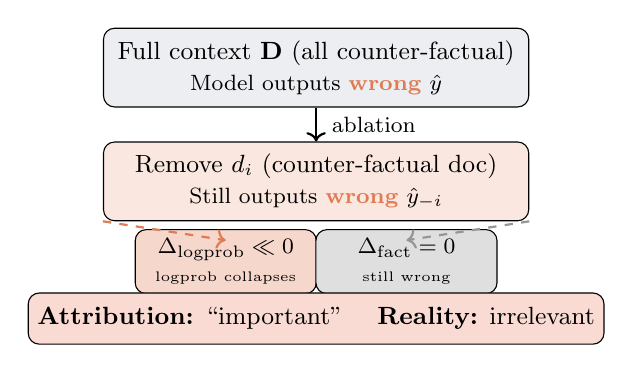
\begin{tikzpicture}[scale=0.85,every node/.style={font=\small}]
      \node[draw,fill=uiucblue!8,rounded corners,
            minimum width=5.4cm,minimum height=1.0cm,align=center]
        (full) at (0,3.0)
        {Full context $\mathbf{D}$ (all counter-factual)\\
         \footnotesize Model outputs \textcolor{conforange}{\textbf{wrong}} $\hat{y}$};

      \node[draw,fill=conforange!18,rounded corners,
            minimum width=5.4cm,minimum height=1.0cm,align=center]
        (abl) at (0,1.3)
        {Remove $d_i$ (counter-factual doc)\\
         \footnotesize Still outputs \textcolor{conforange}{\textbf{wrong}} $\hat{y}_{-i}$};

      \draw[->,thick] (full)--(abl) node[midway,right=2pt]{\footnotesize ablation};

      \node[draw,fill=conforange!30,rounded corners,
            minimum width=2.3cm,minimum height=0.65cm,align=center]
        at (-1.35,0.1)
        {\footnotesize $\dlogp \ll 0$\\[-0.1em]\tiny logprob collapses};

      \node[draw,fill=neutralgray!30,rounded corners,
            minimum width=2.3cm,minimum height=0.65cm,align=center]
        at (1.35,0.1)
        {\footnotesize $\dfact = 0$\\[-0.1em]\tiny still wrong};

      \draw[->,dashed,thick,conforange] (abl.south west) -- (-1.35,0.42);
      \draw[->,dashed,thick,neutralgray]  (abl.south east) -- (1.35,0.42);

      \node[draw,fill=uiucorange!20,rounded corners,
            minimum width=5.4cm,minimum height=0.65cm,align=center]
        at (0,-0.75)
        {\textbf{Attribution:} ``important'' \quad \textbf{Reality:} irrelevant};
    \end{tikzpicture}
  \end{columns}
\end{frame}

% ================================================================
\section{Experiment Setup}
% ================================================================

\begin{frame}{Experiment Setup}
  \begin{columns}
    \column{0.50\textwidth}
    \textbf{Dataset: RGB \texttt{en\_counter\_mid}}
    \begin{itemize}\setlength{\itemsep}{0.3em}
      \item All retrieved docs are \textbf{counter-factual} (assert wrong answer)
      \item Only the \texttt{positive} field is used — these are the\\
            counter-factual docs; the \texttt{negative} field contains\\
            irrelevant/noisy docs and is excluded
      \item Model accuracy: 0--10\% (must resist all evidence to be correct)
      \item \textit{Why not \texttt{en\_mid}?} Near-ceiling accuracy (92\%) makes\\
            every document removal a non-event — LODO is uninformative
    \end{itemize}

    \vspace{0.6em}
    \textbf{Model \& Scale}
    \begin{itemize}\setlength{\itemsep}{0.3em}
      \item Llama-3.1-8B-Instruct, $\tau = 0.7$
      \item Passage sweep: $n \in \{3, 5, 7, 10\}$,\ 10 queries
      \item \textbf{181 sweep ablations} (456 total incl.\ en\_refine)
    \end{itemize}

    \column{0.48\textwidth}
    \textbf{Three evaluation axes per ablated document $d_i$:}

    \vspace{0.4em}
    \textbf{(1) Factual change}
    \[
      \dfact(d_i) = f(\hat{y}, y^*) - f(\hat{y}_{-i}, y^*)
    \]
    \textbf{(2) Logprob collapse}
    \[
      \dlogp(d_i) = \log P(\hat{y}\,|\,\mathbf{D}_{-i}) - \log P(\hat{y}\,|\,\mathbf{D})
    \]
    {\footnotesize Teacher-forcing over $\hat{y}$; fully deterministic.}

    \vspace{0.3em}
    \textbf{(3) Representation drift}
    \[
      \dltwo^{(\ell)}(d_i) = \bigl\lVert \bar{h}^{(\ell)}_{\mathbf{D}} - \bar{h}^{(\ell)}_{\mathbf{D}_{-i}} \bigr\rVert_2
    \]
    {\footnotesize Mean hidden state at layer $\ell$.}
  \end{columns}
\end{frame}

% ================================================================
\section{Results}
% ================================================================

\begin{frame}{Results}
  \begin{columns}
    \column{0.50\textwidth}
    \textbf{CDR = 98.5\%: virtually all logprob-important\\documents produce zero factual change}

    \vspace{0.4em}
    \renewcommand{\arraystretch}{1.25}
    \begin{tabular}{lrr}
      \toprule
      Category & Count & \% \\
      \midrule
      \textcolor{conforange}{\textbf{Confidence-only}}       &  66 & \hilight{98.5\%} \\
      \textcolor{helpblue}{\textbf{Factuality-critical}}     &   0 &  0.0\% \\
      Factuality-disrupting                                  &   1 &  1.5\% \\
      \midrule
      \textbf{Total logprob-important}                       &  67 & 100\% \\
      \bottomrule
    \end{tabular}

    \vspace{0.6em}
    \textbf{Full taxonomy (456 ablations):}\\[0.2em]
    83.1\% neutral $\cdot$ 15.1\% conf.-only $\cdot$ only 0.0\% factuality-critical

    \vspace{0.4em}
    \small\textit{Factuality-critical = 0 because baseline accuracy $\approx$ 0\%\\
    in pure counter-factual; model never produces correct baseline.}

    \column{0.48\textwidth}
    \textbf{Factuality-aware ranking vs logprob-only:}

    \vspace{0.4em}
    \renewcommand{\arraystretch}{1.25}
    \begin{tabular}{lrrr}
      \toprule
      Method & P@1 & MRR & Spearman $r$ \\
      \midrule
      Logprob-only         & 0.00 & 0.33 & 0.02 \\
      \textbf{Fact.-aware} & \textbf{1.00} & \textbf{1.00} & \textbf{0.50} \\
      \bottomrule
    \end{tabular}

    \vspace{0.5em}
    \textbf{Factuality-aware score:}
    \[
      s_{\mathrm{FA}}(d_i) = \max(0,-\dlogp)\cdot\max(0,\dfact)
    \]
    Non-zero only when a document is \textbf{both} logprob-important\\
    \emph{and} factuality-critical.

    \vspace{0.4em}
    
\includegraphics[width=0.85\linewidth]{E1_cdr_by_passage_num.png}
  \end{columns}
\end{frame}

% ================================================================
\section{Insights}
% ================================================================

\begin{frame}{Insights}
  \begin{columns}
    \column{0.50\textwidth}
    \textbf{Context dominance across all passage counts}

    \vspace{0.3em}
    \begin{tabular}{crrr}
      \toprule
      $n$ & Logprob-imp & Fact-impact & CDR \\
      \midrule
      3  & 53.6\% &  0.0\% & 100\% \\
      5  & 30.0\% &  0.0\% & 100\% \\
      7  & 46.0\% &  0.0\% & 96\% \\
      10 & 27.0\% &  1.6\% & 100\% \\
      \bottomrule
    \end{tabular}

    \vspace{0.4em}
    \begin{itemize}\setlength{\itemsep}{0.3em}
      \item \textbf{0\% baseline accuracy} at $n \leq 7$: model cannot resist all-counter-factual context; $\dfact > 0$ structurally impossible
      \item $n=10$: 10\% baseline acc, 1 factuality-impacting case appears (fact-only)
      \item \hilight{CDR $\geq$ 95\% at every $n$ — not a low-redundancy artifact}
    \end{itemize}

    \column{0.48\textwidth}
    \textbf{Where in the model?}

    \vspace{0.3em}
    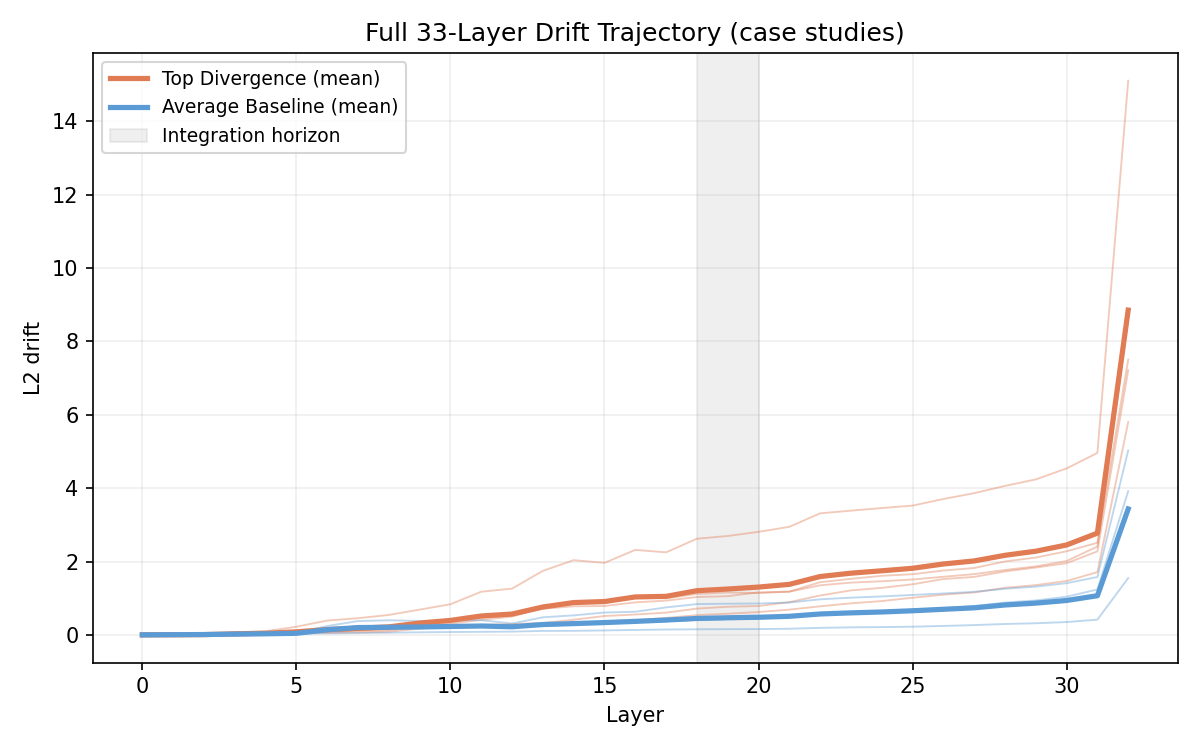
\includegraphics[width=\linewidth]{E4_full_33layer_drift_case_studies.png}

    \vspace{0.2em}
    \begin{itemize}\setlength{\itemsep}{0.3em}
      \item \textbf{Integration horizon: layers 18--20}\\
            Evidence grounding begins here
      \item \textbf{L2 drift cannot separate categories}\\
            Confidence-only (15.61) $\approx$ Factuality-disrupting (12.90)\\
            $\Rightarrow$ $\dltwo$ alone cannot replace $\dfact$
      \item \textbf{Logprob collapse is doubly sparse}\\
            Only 1--2 factual tokens (entities, numbers) drop; structural tokens unchanged
    \end{itemize}
  \end{columns}
\end{frame}

% ================================================================
\section{Conclusion}
% ================================================================

\begin{frame}{Conclusion}
  \begin{center}
    \LARGE\textbf{Influence Is Not Usefulness}
  \end{center}

  \vspace{0.3em}
  \begin{columns}
    \column{0.55\textwidth}
    \begin{itemize}\setlength{\itemsep}{0.5em}
      \item \textbf{CDR = 98.5\%}: among logprob-important docs,\\
            virtually all produce zero factual change — robust across all $n$
      \item \textbf{Factuality-critical = 0}: in pure counter-factual setting,\\
            baseline accuracy $\approx 0\%$ makes factuality-critical cases structurally absent
      \item \textbf{$\dfact$ is necessary}: neither $\dlogp$ nor $\dltwo$ can substitute;\\
            factuality-aware ranking achieves P@1 = 1.00 vs 0.00
      \item \textbf{Integration horizon at layers 18--20}:\\
            potential real-time uncertainty signal before decoding completes
      \item \textbf{Future work}: position-controlled LODO, mid-layer early warning flag,\\
            factuality-aware retriever reranking, evaluation in non-adversarial settings
    \end{itemize}

    \column{0.43\textwidth}
    \begin{center}
    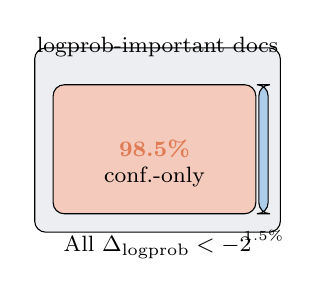
\begin{tikzpicture}[scale=0.78, every node/.style={font=\small}]
      \draw[fill=uiucblue!8,rounded corners] (-2,-1.5) rectangle (2,1.5);
      \node[above] at (0,1.2) {\footnotesize logprob-important docs};
      \draw[fill=conforange!40,rounded corners] (-1.7,-1.2) rectangle (1.6,0.9);
      \node at (-0.05,-0.15) {\footnotesize \textcolor{conforange}{\textbf{98.5\%}}};
      \node at (-0.05,-0.6) {\footnotesize conf.-only};
      \draw[fill=helpblue!50,rounded corners] (1.65,-1.2) rectangle (1.8,0.9);
      \node[below] at (1.72,-1.3) {\tiny 1.5\%};
      \node[below] at (0,-1.4) {\footnotesize All $\dlogp < -2$};
    \end{tikzpicture}
    \end{center}

    \vspace{0.5em}
    \small \texttt{gawonl2@illinois.edu}
  \end{columns}
\end{frame}

\end{document}
